\section{Cực trị của hàm số}
\label{sec:extrema-of-functions}

Một trong những ứng dụng quan trọng nhất của phép tính vi phân là giải quyết các bài toán tối ưu hóa. Các bài toán này yêu cầu chúng ta tìm ra phương án ``tốt nhất'' trong một tập hợp các khả năng, chẳng hạn như tối đa hóa lợi nhuận, tối thiểu hóa chi phí, hoặc tìm ra quãng đường ngắn nhất. Về mặt toán học, nhiều bài toán tối ưu hóa có thể được quy về việc tìm giá trị lớn nhất (maximum) và giá trị nhỏ nhất (minimum) của một hàm số trên một tập xác định cho trước.

\begin{definition}[Cực trị của hàm số]\label{def:extrema}
Cho hàm số $f$ xác định trên tập $D \subset \R$ và $c \in D$.
\begin{enumerate}[label=(\alph*)]
    \item Ta nói $f$ có \textbf{cực đại toàn cục} (global maximum) hay \textbf{giá trị lớn nhất} tại $c$ nếu $f(c) \ge f(x)$ với mọi $x$ thuộc $D$.
    \item Ta nói $f$ có \textbf{cực tiểu toàn cục} (global minimum) hay \textbf{giá trị nhỏ nhất} tại $c$ nếu $f(c) \le f(x)$ với mọi $x$ thuộc $D$.
    \item Ta nói $f$ có \textbf{cực đại địa phương} (local maximum) tại $c$ nếu tồn tại một khoảng mở $(a,b) \subset D$ chứa $c$ sao cho $f(c) \ge f(x)$ với mọi $x$ thuộc $(a,b)$.
    \item Ta nói $f$ có \textbf{cực tiểu địa phương} (local minimum) tại $c$ nếu tồn tại một khoảng mở $(a,b) \subset D$ chứa $c$ sao cho $f(c) \le f(x)$ với mọi $x$ thuộc $(a,b)$.
\end{enumerate}
\end{definition}

Các giá trị lớn nhất/nhỏ nhất và cực đại/cực tiểu địa phương được gọi chung là \textbf{giá trị cực trị} (extreme values), và điểm $c$ nơi chúng xảy ra được gọi là \textbf{điểm cực trị} (extremum point). Cần phân biệt rằng cực trị toàn cục (hay tuyệt đối) được xét trên toàn bộ miền xác định $D$, trong khi cực trị địa phương (hay tương đối) chỉ cần xét trong một lân cận nhỏ quanh điểm đó.

Một cách trực quan, trên đồ thị của hàm số, điểm cực đại toàn cục là điểm ``cao nhất'' trên toàn bộ đồ thị, trong khi điểm cực đại địa phương là điểm ``cao nhất'' so với các điểm lân cận nó (xem Hình \ref{fig:extrema-example}). Theo định nghĩa, một giá trị cực trị toàn cục nếu không xảy ra ở biên của miền xác định thì nó cũng là một giá trị cực trị địa phương.

\begin{figure}[H]
    \centering
    \begin{tikzpicture}
        \begin{axis}[
            axis lines=middle,
            xlabel=$x$,
            ylabel=$y$,
            xtick={-3, -1, 1, 2, 4},
            xticklabels={$a$, $b$, $c$, $d$, $e$},
            ytick={-1.5, -1, 1, 3.5, 5},
            yticklabels={},
            ymin=-2, ymax=6,
            xmin=-4, xmax=5,
            width=12cm,
            height=8cm,
        ]
        \addplot[smooth, thick, myblue, domain=-3:1] {
            -1/4*x^3 + 3/8*x^2+3/2*x-5/8
        } node[pos=0.9, right] {};
        \addplot[smooth, thick, myblue, domain=1:3.5] {
            2*x^2 - 8*x + 7
        } node[pos=0.9, right] {};
        % \addplot[smooth, thick, myblue, domain=-3.5:2] {
        %     -0.1x^3 - 3x^2
        % };

        % Các điểm cực trị
        \node[circle, fill=myblue, inner sep=1.5pt] at (axis cs:-3, 5) {};
        \node[circle, fill=myblue, inner sep=1.5pt] at (axis cs:-1, -1.5) {};
        \node[circle, fill=myblue, inner sep=1.5pt] at (axis cs:1, 1) {};
        \node[circle, fill=myblue, inner sep=1.5pt] at (axis cs:2, -1) {};
        \node[circle, fill=myblue, inner sep=1.5pt] at (axis cs:3.5, 3.5) {};

        % Đường gióng
        \draw[dashed] (axis cs:-3, 0) -- (axis cs:-3, 5) -- (axis cs:0, 5);
        \draw[dashed] (axis cs:-1, 0) -- (axis cs:-1, -1.5) -- (axis cs:0, -1.5);
        \draw[dashed] (axis cs:1, 0) -- (axis cs:1, 1) -- (axis cs: 0, 1);
        \draw[dashed] (axis cs:2, 0) -- (axis cs:2, -1) -- (axis cs:0, -1);
        \draw[dashed] (axis cs:3.5, 0) -- (axis cs:3.5, 3.5) -- (axis cs:0, 3.5);

        \node at (axis cs: 0, 5) [right] {$f(a)$};
        \node at (axis cs:0, 3.5) [left] {$f(e)$};
        \node at (axis cs: 0, 1) [left] {$f(c)$};
        \node at (axis cs: 0, -1.5) [right] {$f(b)$};
        \node at (axis cs: 0, -1) [above right] {$f(d)$};
        \end{axis}
    \end{tikzpicture}
    \caption{\centering Cực tiểu tuyệt đối $f(b)$, không có cực đại tuyệt đối, cực tiểu địa phương $f(b)$ và $f(d)$, cực đại địa phương $f(c)$.}
    \label{fig:extrema-example}
\end{figure}

\begin{example}\label{ex:parabola-extrema}
Xét hàm số $f(x) = x^2$ trên miền xác định $\R$ (xem Hình \ref{fig:parabola-extrema}). Vì $f(x) = x^2 \ge 0 = f(0)$ với mọi $x \in \R$, hàm số đạt \textbf{cực tiểu toàn cục} (cũng là cực tiểu địa phương) bằng 0 tại $x=0$. Tuy nhiên, đồ thị của hàm là một parabol không có điểm cao nhất, do đó hàm số không có giá trị cực đại.

Nếu ta giới hạn miền xác định trên đoạn $[-1, 2]$, hàm số có một cực tiểu địa phương tại $x=0$, một cực tiểu toàn cục tại $x=0$, và một cực đại toàn cục tại $x=2$ (với giá trị $f(2)=4$). Hàm không có cực đại địa phương trong trường hợp này.
\end{example}

\begin{figure}[H]
    \centering
    \begin{tikzpicture}
        \begin{axis}[
            axis lines=middle,
            xlabel=$x$,
            ylabel=$y$,
            ymin=-1, ymax=5,
            xmin=-3, xmax=3,
            width=10cm,
            height=7cm,
        ]
        \addplot[domain=-2.2:2.2, samples=100, thick, myblue] {x^2} node[pos=0.8, right, black] {$f(x)=x^2$};
        \end{axis}
    \end{tikzpicture}
    \caption{Hàm số $f(x)=x^2$ có giá trị cực tiểu là 0, không có giá trị cực đại.}
    \label{fig:parabola-extrema}
\end{figure}

\begin{example}\label{ex:cubic-no-extrema}
Hàm số $f(x) = x^3$ không có cực trị trên $\R$. Đồ thị của hàm số này luôn đi lên, do đó không tồn tại điểm nào cao nhất hay thấp nhất, cả trên phương diện toàn cục lẫn địa phương (xem Hình \ref{fig:cubic-no-extrema}).
\end{example}

\begin{figure}[H]
    \centering
    \begin{tikzpicture}
        \begin{axis}[
            axis lines=middle,
            xlabel=$x$,
            ylabel=$y$,
            xtick=null,
            ytick=null,
            ymin=-5, ymax=5,
            xmin=-2, xmax=2,
            width=8cm,
            height=8cm,
            elapsed=false,
        ]
        \addplot[domain=-1.7:1.7, samples=100, thick, myblue] {x^3} node[pos=0.9, right, black] {$f(x)=x^3$};
        \end{axis}
    \end{tikzpicture}
    \caption{Hàm số $f(x)=x^3$ không có cực trị.}
    \label{fig:cubic-no-extrema}
\end{figure}

Quan sát các đồ thị, ta thấy rằng nếu một hàm số đạt cực trị địa phương tại một điểm trong miền xác định và có tiếp tuyến tại điểm đó, thì tiếp tuyến này phải nằm ngang. Điều này dẫn đến một kết quả then chốt sau đây.

\begin{theorem}[Định lý Fermat]
\label{thm:fermat}
Nếu hàm số $f$ có một cực trị địa phương tại $c$ và $f'(c)$ tồn tại, thì $f'(c) = 0$.
\end{theorem}

Định lý Fermat khẳng định rằng tại một điểm cực trị địa phương (không phải điểm biên), nếu hàm số khả vi thì đạo hàm phải bằng không. Đây là một trong những ứng dụng nền tảng nhất của đạo hàm trong việc tìm kiếm các điểm tối ưu.

\begin{proof}
Giả sử $f$ có một cực đại địa phương tại $c$. Theo định nghĩa, tồn tại một khoảng mở chứa $c$ sao cho $f(c) \ge f(c+h)$ với mọi $h$ đủ nhỏ (cả dương và âm).
\begin{itemize}
    \item Nếu $h > 0$ và đủ nhỏ, ta có $f(c+h) - f(c) \le 0$. Do đó, tỉ số $\dfrac{f(c+h) - f(c)}{h} \le 0$. Lấy giới hạn khi $h \to 0^+$, ta được:
    $$f'(c) = \limit{h}{0^+} \dfrac{f(c+h) - f(c)}{h} \le 0.$$
    \item Nếu $h < 0$ và đủ nhỏ, ta vẫn có $f(c+h) - f(c) \le 0$. Tuy nhiên, vì $h < 0$, tỉ số $\dfrac{f(c+h) - f(c)}{h} \ge 0$. Lấy giới hạn khi $h \to 0^-$, ta được:
    $$f'(c) = \limit{h}{0^-} \dfrac{f(c+h) - f(c)}{h} \ge 0.$$
\end{itemize}
Vì $f'(c)$ vừa không dương vừa không âm, ta buộc phải có $f'(c) = 0$.

Chứng minh cho trường hợp $f$ có cực tiểu địa phương tại $c$ được thực hiện một cách tương tự.
\end{proof}

Một điểm $c$ trong miền xác định của $f$ mà tại đó $f'(c)=0$ được gọi là một \textbf{điểm dừng} (stationary point). Một điểm $c$ mà tại đó $f'(c)=0$ hoặc $f'(c)$ không tồn tại được gọi là một \textbf{điểm tới hạn} (critical point) của hàm số.

\begin{example}\label{ex:abs-critical-point}
Hàm số $f(x) = \abs{x}$ có một điểm tới hạn tại $x=0$ vì $f'(0)$ không tồn tại (như đã thấy ở Ví dụ 3.1.10).
\end{example}

Từ Định lý Fermat, ta có thể phát biểu lại một cách ngắn gọn: một hàm số chỉ có thể đạt cực trị địa phương tại các điểm tới hạn của nó.

\begin{example}\label{ex:quartic-extrema}
Tìm giá trị nhỏ nhất của hàm số $f(x) = x^4 - 6x^2 - 10$.
\begin{figure}[H]
    \centering
    \begin{tikzpicture}
        \begin{axis}[
            axis lines=middle,
            xlabel=$x$,
            ylabel=$y$,
            ymin=-20, ymax=40,
            xmin=-4.5, xmax=4.5,
            width=12cm,
            height=8cm,
            grid=major,
        ]
        \addplot[domain=-4:4, samples=200, thick, myblue] {x^4 - 6*x^2 - 10};
        \end{axis}
    \end{tikzpicture}
    \caption{Đồ thị hàm $f(x) = x^4 - 6x^2 - 10$.}
    \label{fig:quartic-extrema}
\end{figure}

Từ đồ thị (Hình \ref{fig:quartic-extrema}), ta có thể dự đoán hàm số có giá trị nhỏ nhất. Vì miền xác định là $\R$ (một tập mở), điểm mà tại đó $f$ đạt cực tiểu toàn cục cũng phải là một điểm cực tiểu địa phương. Theo Định lý Fermat, điểm này phải là một điểm dừng. Ta tiến hành giải phương trình $f'(x) = 0$:
$$ f'(x) = 4x^3 - 12x = 0 \iff 4x(x^2 - 3) = 0 $$
Phương trình có các nghiệm $x=0$, $x=\sqrt{3}$, và $x=-\sqrt{3}$. Đây là tất cả các điểm tới hạn của hàm số.

Ta tính giá trị của hàm tại các điểm này:
\begin{itemize}
    \item $f(0) = -10$
    \item $f(\sqrt{3}) = (\sqrt{3})^4 - 6(\sqrt{3})^2 - 10 = -19$
    \item $f(-\sqrt{3}) = (-\sqrt{3})^4 - 6(-\sqrt{3})^2 - 10 = -19$
\end{itemize}
So sánh các giá trị, ta kết luận giá trị nhỏ nhất của hàm số là $-19$, xảy ra tại $x=\sqrt{3}$ và $x=-\sqrt{3}$.
\end{example}

\subsection{Sự tồn tại giá trị lớn nhất và giá trị nhỏ nhất}
\label{sec:existence-global-extrema}

Định lý Fermat cho chúng ta biết nơi để tìm kiếm các điểm cực trị địa phương, nhưng nó không đảm bảo sự tồn tại của các điểm đó, cũng như không đề cập đến cực trị toàn cục. Dưới đây là một định lý nền tảng đảm bảo sự tồn tại của cực trị toàn cục trong một điều kiện rất phổ biến.

\begin{theorem}[Định lý Cực trị Toàn cục]\label{thm:extreme-value-theorem}
Nếu hàm số $f$ liên tục trên một đoạn đóng $[a, b]$, thì $f$ chắc chắn đạt được giá trị lớn nhất toàn cục và giá trị nhỏ nhất toàn cục trên đoạn đó.
\end{theorem}

Nói một cách ngắn gọn: \textit{Một hàm liên tục trên một đoạn đóng thì luôn có giá trị lớn nhất và nhỏ nhất.}

Định lý này là một hệ quả sâu sắc của tính đầy đủ của tập hợp số thực. Chứng minh chi tiết của nó có thể được tìm thấy trong các giáo trình giải tích nâng cao. [Kha96, tr. 56]

Từ định lý trên, ta thấy rằng cực trị toàn cục của một hàm liên tục trên đoạn $[a,b]$ có thể xảy ra tại:
\begin{enumerate}
    \item Các điểm tới hạn nằm \textbf{bên trong} khoảng mở $(a,b)$.
    \item Hai điểm \textbf{biên} là $a$ và $b$.
\end{enumerate}

\begin{figure}[H]
    \centering
    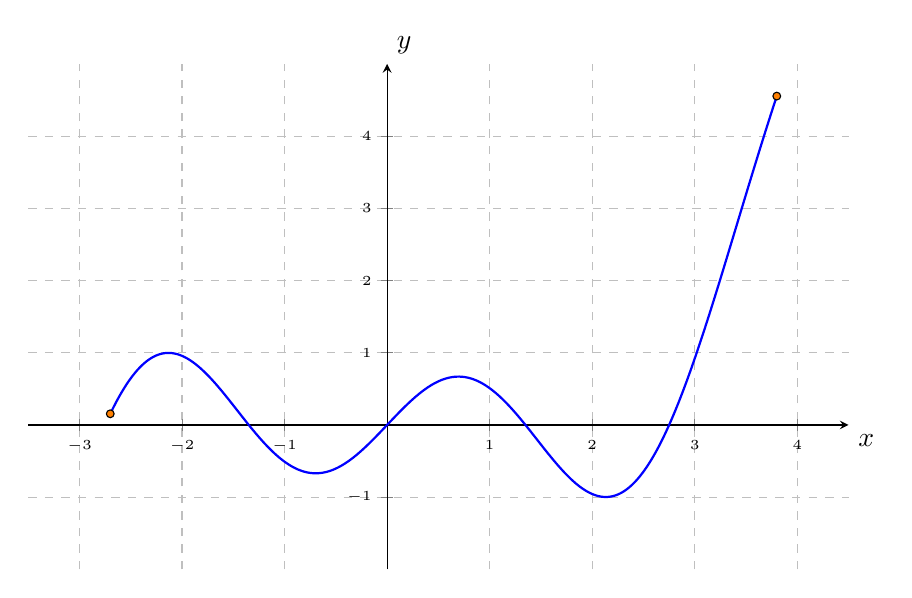
\begin{tikzpicture}
        % \begin{axis}[
        %     axis lines=middle,
        %     grid=major, % Giữ lại grid major nếu muốn
        %     grid style={dashed, gray!50}, % Thêm style cho grid: nét đứt, màu xám nhạt
        %     xmin=-3.5, xmax=4.5,
        %     ymin=-2, ymax=4,
        %     xtick=\empty, % Ẩn các số trên trục x
        %     ytick=\empty, % Ẩn các số trên trục y
        %     enlargelimits=false,
        %     axis line style={-},
        % ]
        \begin{axis}[
            axis lines=middle,
            xlabel=$x$,
            ylabel=$y$,
            xmin=-3.5, xmax=4.5,
            ymin=-2, ymax=5,
            grid=major,
            grid style={dashed, gray!50},
            xtick={-3, -2,-1,...,4},
            ytick={-1,0,1,...,4},
            % xtick=\empty,
            % ytick=\empty,
            width=12cm,
            height=8cm,
            tick label style={font=\tiny},
            xlabel style={anchor=north west},
            ylabel style={anchor=south west},
            no markers % Tắt các marker tự động
        ]
        % Vẽ đồ thị hàm số uốn lượn
        % Hàm số được chọn để có hình dáng tương tự hình gốc
        \addplot[
            domain=-2.7:3.8, 
            samples=150, 
            color=blue, 
            thick,
            smooth,
        ] {sin(deg(2*x)) + 0.1*x^3 - 0.5*x};

        % Đánh dấu 2 điểm đầu mút
        \addplot[
            mark=*,
            mark options={fill=orange, scale=0.7},
            only marks,
        ] coordinates {
            (-2.7, {sin(deg(2*(-2.7))) + 0.1*(-2.7)^3 - 0.5*(-2.7)})
            (3.8, {sin(deg(2*3.8)) + 0.1*(3.8)^3 - 0.5*(3.8)})
        };
        
        \end{axis}
    \end{tikzpicture}
    \caption{Cực trị toàn cục xảy ra ở điểm dừng hoặc trên biên.}
    \label{fig:cuc-tri-toan-cuc-dashed-grid}
\end{figure}

Kết hợp các nhận định trên, ta có một quy trình rõ ràng để tìm giá trị lớn nhất và nhỏ nhất của một hàm liên tục trên một đoạn đóng.

\begin{importantbox}
    \textbf{Quy trình tìm cực trị toàn cục trên đoạn đóng $[a,b]$}
    \begin{enumerate}
    \item \textbf{Bước 1:} Tìm tất cả các điểm tới hạn của $f$ trong khoảng mở $(a,b)$.
    \item \textbf{Bước 2:} Tính giá trị của $f$ tại các điểm tới hạn tìm được ở Bước 1 và tại hai điểm biên $a$ và $b$.
    \item \textbf{Bước 3:} So sánh tất cả các giá trị tính được ở Bước 2. Giá trị lớn nhất là giá trị lớn nhất toàn cục, và giá trị nhỏ nhất là giá trị nhỏ nhất toàn cục của hàm số trên đoạn $[a,b]$.
    \end{enumerate}
\end{importantbox}

\begin{example}
\label{ex:find-global-extrema-1}
Tìm giá trị lớn nhất và nhỏ nhất của hàm $f(x) = x^4 - 2x^3 - 2x^2 + 5$ trên đoạn $[-1, 3]$.

\textit{Phân tích:} Hàm $f$ là một đa thức nên nó liên tục trên đoạn đóng $[-1,3]$. Do đó, theo Định lý Cực trị Toàn cục, nó chắc chắn có giá trị lớn nhất và nhỏ nhất trên đoạn này.

\textbf{Bước 1:} Tìm các điểm tới hạn. Ta tính đạo hàm:
$$ f'(x) = 4x^3 - 6x^2 - 4x = 2x(2x^2 - 3x - 2) = 2x(2x+1)(x-2) $$
Giải phương trình $f'(x) = 0$, ta được các điểm dừng là $x=0$, $x=2$, và $x = -1/2$. Cả ba điểm này đều nằm trong khoảng mở $(-1,3)$.

\textbf{Bước 2:} Tính giá trị.
\begin{itemize}
    \item Tại các điểm tới hạn: 
        \begin{itemize}
            \item $f(0) = 5$
            \item $f(2) = 16 - 16 - 8 + 5 = -3$
            \item $f(-1/2) = \dfrac{1}{16} - 2(-\dfrac{1}{8}) - 2(\dfrac{1}{4}) + 5 = \dfrac{1}{16} + \dfrac{1}{4} - \dfrac{1}{2} + 5 = \dfrac{79}{16} \approx 4.94$
        \end{itemize}
    \item Tại các điểm biên:
        \begin{itemize}
            \item $f(-1) = 1 - 2(-1) - 2(1) + 5 = 1 + 2 - 2 + 5 = 6$
            \item $f(3) = 81 - 2(27) - 2(9) + 5 = 81 - 54 - 18 + 5 = 14$
        \end{itemize}
\end{itemize}

\textbf{Bước 3:} So sánh.
Các giá trị ta thu được là: $5, -3, 4.94, 6, 14$.

Vậy, trên đoạn $[-1,3]$, giá trị lớn nhất của hàm số là $14$ (đạt tại $x=3$) và giá trị nhỏ nhất là $-3$ (đạt tại $x=2$).
\end{example}

\begin{example}\label{ex:find-global-extrema-2}
Tìm giá trị lớn nhất và nhỏ nhất của hàm $f(x) = x^3 - 9x^2 + 24x - 10$ trên đoạn $[0, 5]$.

\textbf{Bước 1:} Ta có $f'(x) = 3x^2 - 18x + 24 = 3(x^2 - 6x + 8) = 3(x-2)(x-4)$.
Giải $f'(x)=0$, ta được các điểm dừng $x=2$ và $x=4$. Cả hai đều nằm trong khoảng $(0,5)$.

\textbf{Bước 2:} Tính giá trị.
\begin{itemize}
    \item Tại các điểm tới hạn:
        \begin{itemize}
            \item $f(2) = 8 - 9(4) + 24(2) - 10 = 8 - 36 + 48 - 10 = 10$
            \item $f(4) = 64 - 9(16) + 24(4) - 10 = 64 - 144 + 96 - 10 = 6$
        \end{itemize}
    \item Tại các điểm biên:
        \begin{itemize}
            \item $f(0) = -10$
            \item $f(5) = 125 - 9(25) + 24(5) - 10 = 125 - 225 + 120 - 10 = 10$
        \end{itemize}
\end{itemize}
\textbf{Bước 3:} So sánh các giá trị: $10, 6, -10$.

Kết luận: Giá trị lớn nhất là $10$ (xảy ra tại $x=2$ và $x=5$), giá trị nhỏ nhất là $-10$ (xảy ra tại $x=0$).
\end{example}

\subsection{Các định lý giá trị trung bình}
\label{sec:mean-value-theorems}

Các định lý dưới đây đóng vai trò trung tâm trong việc kết nối các tính chất của một hàm số với đạo hàm của nó. Chúng là công cụ lý thuyết nền tảng cho phép chúng ta suy luận về hành vi của hàm số từ thông tin của đạo hàm.

\begin{theorem}[Định lý Rolle]\label{thm:rolle}
Giả sử hàm số $f$ thỏa mãn các điều kiện sau:
\begin{enumerate}[label=(\roman*)]
    \item $f$ liên tục trên đoạn đóng $[a, b]$.
    \item $f$ khả vi trên khoảng mở $(a, b)$.
    \item $f(a) = f(b)$.
\end{enumerate}
Khi đó, tồn tại ít nhất một số thực $c$ thuộc khoảng $(a, b)$ sao cho $f'(c) = 0$.
\end{theorem}

\begin{figure}[H]
    \centering
    \begin{tikzpicture}
        \begin{axis}[
            axis lines=middle,
            xlabel=$x$,
            ylabel=$y$,
            % ticks đặt tại a, c, b
            xtick={1.6,3.3,6.4},
            xticklabels={$a$, $c$, $b$},
            % y-tick cho f(a)=f(b)
            ytick={2.0},
            yticklabels={$f(a)=f(b)$},
            ymin=0, ymax=5,
            xmin=0, xmax=7.6,
            width=12cm,
            height=7cm,
            clip=false,
            every axis x label/.style={at={(axis description cs:1,0.05)},anchor=north west},
            every axis y label/.style={at={(axis description cs:0.02,1)},anchor=south west},
        ]

        % --- đường cong f(x) (dùng coordinates để đảm bảo A,P,B chính xác)
        % A=(1.6,2.0), P=(3.3,3.2), B=(6.4,2.0)
        \addplot[myblue, very thick, smooth, samples=200] coordinates {
            (1.6,2.0) (2.2,2.6) (2.7,3.0)
            (3.0,3.18) (3.3,3.2) (3.6,3.18) (4.2,2.9) (4.9,2.6)
            (5.6,2.25) (6.0,2.08) (6.4,2.0)
        };

        % --- vẽ điểm A, P, B (điểm đen)
        \addplot+[only marks, mark=*, mark size=1.8pt] coordinates {
            (1.6,2.0) (3.3,3.2) (6.4,2.0)
        };
        \node[above left,font=\small]  at (axis cs:1.6,2.0) {A};
        \node[above,font=\small]       at (axis cs:3.3,3.2) {P};
        \node[above right,font=\small] at (axis cs:6.4,2.0) {B};

        % --- tiếp tuyến tại P (đường thẳng ngang, màu hồng)
        \draw[line width=1.6pt, color=magenta] (axis cs:1.9,3.2) -- (axis cs:4.7,3.2);

        % --- đường gióng đứt nét: verticals từ a,c,b lên đồ thị
        \draw[dashed] (axis cs:1.6,0) -- (axis cs:1.6,2.0);
        \draw[dashed] (axis cs:3.3,0) -- (axis cs:3.3,3.2);
        \draw[dashed] (axis cs:6.4,0) -- (axis cs:6.4,2.0);

        % --- đường ngang đứt nét cho f(a)=f(b)
        \draw[dashed] (axis cs:0,2.0) -- (axis cs:6.4,2.0);

        % --- thêm các nét nhỏ trên trục y để biểu diễn tick alignment (như hình)
        \draw (-0.06,2.0) -- (0.06,2.0);

        \end{axis}
    \end{tikzpicture}
    \caption{\centering Minh họa Định lý Rolle: nhìn vào hình ta thấy khi $A$ và $B$ có cùng tung độ, thì động tại tiếp tuyến với một điểm ``ở giữa" đồ thị và song song với $AB$ (đường thẳng nằm ngang đi qua P)}
    \label{fig:rolle-theorem}
\end{figure}

\begin{proof}
Ta xét ba trường hợp có thể xảy ra:
\begin{enumerate}[label=(\alph*)]
    \item \textbf{Trường hợp 1:} $f(x) = f(a)$ với mọi $x \in [a,b]$. Khi đó $f$ là hàm hằng, nên $f'(x) = 0$ với mọi $x \in (a,b)$. Ta có thể chọn $c$ là một điểm bất kỳ trong $(a,b)$.
    \item \textbf{Trường hợp 2:} Tồn tại một điểm $x_0 \in (a,b)$ sao cho $f(x_0) > f(a)$. Vì $f$ liên tục trên đoạn đóng $[a,b]$, theo Định lý Cực trị Toàn cục (\ref{thm:extreme-value-theorem}), $f$ phải đạt giá trị lớn nhất toàn cục tại một điểm $c \in [a,b]$. Vì $f(x_0) > f(a) = f(b)$, điểm $c$ này không thể là $a$ hoặc $b$. Do đó, $c$ phải nằm trong khoảng mở $(a,b)$. Điều này có nghĩa là $f$ đạt cực đại địa phương tại $c$. Vì $f$ khả vi tại $c$, theo Định lý Fermat (\ref{thm:fermat}), ta phải có $f'(c)=0$.
    \item \textbf{Trường hợp 3:} Tồn tại một điểm $x_0 \in (a,b)$ sao cho $f(x_0) < f(a)$. Lập luận tương tự như trường hợp 2, $f$ phải đạt giá trị nhỏ nhất toàn cục tại một điểm $c$ trong khoảng mở $(a,b)$, và tại đó $f'(c)=0$.
\end{enumerate}
\end{proof}

Định lý Rolle có thể được tổng quát hóa cho trường hợp $f(a) \neq f(b)$. Kết quả này, được gọi là Định lý giá trị trung bình, là một trong những công cụ mạnh mẽ và hữu ích nhất của giải tích.

\begin{theorem}[Định lý Giá trị Trung bình - Lagrange]\label{thm:mean-value-theorem}
Nếu hàm số $f$ liên tục trên đoạn $[a, b]$ và khả vi trên khoảng $(a, b)$, thì tồn tại ít nhất một số thực $c \in (a, b)$ sao cho:
$$ f'(c) = \dfrac{f(b) - f(a)}{b - a} $$
\end{theorem}

\begin{figure}[H]
    \centering
    \begin{tikzpicture}
        \begin{axis}[
            axis lines=middle,
            xlabel=$x$,
            ylabel=$y$,
            % đặt ticks tại toạ độ tương ứng của a, c, b
            xtick={1.2,3.3,6.4},
            xticklabels={$a$, $c$, $b$},
            % y-ticks tại f(b) (thấp) và f(a) (cao)
            ytick={1.1,2.1},
            yticklabels={$f(b)$, $f(a)$},
            ymin=0, ymax=3.6,
            xmin=0, xmax=7.6,
            width=12cm,
            height=7cm,
            clip=false,
            every axis x label/.style={at={(axis description cs:1,0.05)},anchor=north west},
            every axis y label/.style={at={(axis description cs:0.02,1)},anchor=south west},
        ]
        %--- Định nghĩa các điểm (theo axis coordinates)
        % A = (1.2, 2.1), P = (3.3, 3.0), B = (6.4, 1.1)
        %
        % Đồ thị f(x) vẽ bằng danh sách toạ độ để đảm bảo A,P,B nằm chính xác trên đồ thị
        \addplot[myblue, thick, smooth, samples=200] coordinates {
          (1.2,2.1) (1.8,2.6) (2.4,2.9)
          (2.9,3.0) (3.3,3.0) (3.7,2.9) (4.3,2.5) (5.2,1.9)
          (5.8,1.4) (6.2,1.2) (6.4,1.1)
        };

        % Vẽ các điểm A, P, B (dấu chấm đen)
        \addplot+[only marks, mark=*, mark size=1.6pt] coordinates {
            (1.2,2.1) (3.3,3.0) (6.4,1.1)
        };
        % Gắn nhãn cho các điểm
        \node[above left] at (axis cs:1.2,2.1) {A};
        \node[above right] at (axis cs:3.3,3.0) {P};
        \node[right] at (axis cs:6.4,1.2) {B};

        %--- Cát tuyến AB (đoạn thẳng nối A và B)
        % Tính hệ số góc: m = (1.1 - 2.1) / (6.4 - 1.2) = -0.1923076923
        % Phương trình: y = m*x + b_chord với b_chord ≈ 2.3307692308
        \addplot[domain=1.2:6.4, thick, black] {-0.1923076923076923*x + 2.3307692307692306};

        %--- Tiếp tuyến tại P: cùng độ dốc với AB (vì muốn song song)
        % Phương trình tiếp tuyến tại P (3.3,3.0): y = m*x + b_tan, 
        % b_tan = 3.0 - m*3.3 ≈ 3.6346153846153846
        \addplot[domain=0.2:6.6, thick, magenta] {-0.1923076923076923*x + 3.6346153846153846};

        %--- Các đường gióng đứt nét (verticals từ a,c,b lên đồ thị; horizontals tới trục y)
        % Verticals
        \draw[dashed] (axis cs:1.2,0) -- (axis cs:1.2,2.1); % a up to A
        \draw[dashed] (axis cs:3.3,0) -- (axis cs:3.3,3.0); % c up to P
        \draw[dashed] (axis cs:6.4,0) -- (axis cs:6.4,1.1); % b up to B
        % Horizontals to y-axis (align f(a) and f(b) to left axis)
        \draw[dashed] (axis cs:0,2.1) -- (axis cs:1.2,2.1); % f(a)
        \draw[dashed] (axis cs:0,1.1) -- (axis cs:6.4,1.1); % f(b) (draw long so visible)
        
        % Một chút chỉnh để các đường ngang nhỏ xuất hiện trên trục y
        \draw (-0.06,2.1) -- (0.06,2.1);
        \draw (-0.06,1.1) -- (0.06,1.1);
        
        \end{axis}
    \end{tikzpicture}
    \caption{\centering Minh họa ý nghĩa hình học của Định lý giá trị trung bình Lagrange: hệ số góc của cát tuyến $AB$ là $\dfrac{f(b)-f(a)}{b-a}$ và có ít nhất một điểm $P$ sao cho tiếp tuyến tại điểm đó song song với cát tuyến $AB$.}
    \label{fig:lagrange-theorem}
\end{figure}

Về mặt hình học, định lý này khẳng định rằng luôn tồn tại một điểm $P$ trên đồ thị của hàm số $f$ mà tại đó tiếp tuyến song song với đường cát tuyến nối hai điểm đầu mút $A(a, f(a))$ và $B(b, f(b))$. Định lý Rolle chính là trường hợp đặc biệt khi cát tuyến AB nằm ngang.

\begin{proof}
Ý tưởng của chứng minh là áp dụng Định lý Rolle cho một hàm phụ được xây dựng một cách khéo léo. Xét hàm số:
$$ g(x) = f(x) - \left[ f(a) + \dfrac{f(b) - f(a)}{b - a}(x-a) \right] $$
Hàm $g(x)$ biểu diễn hiệu số tung độ giữa điểm trên đồ thị $y=f(x)$ và điểm tương ứng trên đường thẳng cát tuyến AB. Ta dễ dàng kiểm tra rằng:
\begin{itemize}
    \item $g$ liên tục trên $[a,b]$ và khả vi trên $(a,b)$.
    \item $g(a) = f(a) - f(a) = 0$.
    \item $g(b) = f(b) - [f(a) + (f(b)-f(a))] = 0$.
\end{itemize}
Vì $g(a) = g(b) = 0$, hàm $g$ thỏa mãn các điều kiện của Định lý Rolle. Do đó, tồn tại $c \in (a,b)$ sao cho $g'(c) = 0$.
Ta có $g'(x) = f'(x) - \dfrac{f(b) - f(a)}{b - a}$.
Vậy, tại điểm $c$, ta có $f'(c) - \dfrac{f(b) - f(a)}{b - a} = 0$, suy ra điều phải chứng minh.
\end{proof}

Một hệ quả trực tiếp và cực kỳ quan trọng của Định lý Giá trị Trung bình là:

\begin{corollary}\label{cor:zero-derivative}
Nếu $f'(x) = 0$ với mọi $x$ trong một khoảng $(a, b)$, thì $f$ là một hàm hằng trên khoảng đó.
\end{corollary}
\begin{proof}
Lấy hai điểm bất kỳ $x_1, x_2$ trong khoảng $(a,b)$ với $x_1 < x_2$. Áp dụng Định lý Giá trị Trung bình trên đoạn $[x_1, x_2]$, tồn tại $c \in (x_1, x_2)$ sao cho:
$$ f(x_2) - f(x_1) = f'(c)(x_2 - x_1) $$
Vì $f'(c) = 0$ theo giả thiết, ta có $f(x_2) - f(x_1) = 0$, hay $f(x_2) = f(x_1)$. Điều này đúng với mọi cặp điểm trong khoảng, do đó $f$ là hàm hằng.
\end{proof}

\begin{corollary}\label{cor:same-derivative}
Nếu $f'(x) = g'(x)$ với mọi $x$ trong một khoảng $(a, b)$, thì tồn tại một hằng số $C$ sao cho $f(x) = g(x) + C$ trên khoảng đó.
\end{corollary}
\begin{proof}
Xét hàm $h(x) = f(x) - g(x)$. Ta có $h'(x) = f'(x) - g'(x) = 0$ trên $(a,b)$. Theo hệ quả trên, $h(x) = C$ với $C$ là một hằng số.
\end{proof}

Định lý Giá trị Trung bình còn có một dạng tổng quát hơn, gọi là Định lý Giá trị Trung bình Cauchy.

\begin{theorem}[Định lý Giá trị Trung bình Cauchy]\label{thm:cauchy-mean-value}
Nếu hai hàm số $f$ và $g$ cùng liên tục trên $[a, b]$ và khả vi trên $(a, b)$, thì tồn tại một điểm $c \in (a, b)$ sao cho:
$$ [f(b) - f(a)]g'(c) = [g(b) - g(a)]f'(c) $$
Nếu $g'(x) \neq 0$ với mọi $x \in (a,b)$, thì ta có thể viết lại dưới dạng:
$$ \dfrac{f(b) - f(a)}{g(b) - g(a)} = \dfrac{f'(c)}{g'(c)} $$
\end{theorem}

\begin{proof}
Áp dụng Định lý Rolle cho hàm số $h(x) = [f(b) - f(a)]g(x) - [g(b) - g(a)]f(x)$.
\end{proof}

\subsection{Bài tập}

\begin{exercise}
Tìm tất cả các điểm tới hạn của các hàm số sau:
\begin{enumerate}[label=(\alph*)]
    \item $f(x) = 2x^3 + 3x^2 - 12x + 1$
    \item $g(t) = t^5 - 5t^3 + 10$
    \item $h(p) = \dfrac{p-1}{p^2+3}$
    \item $f(x) = x^{2/3}(x-5)$
    \item $g(x) = |2x-5|$
\end{enumerate}
\end{exercise}

\begin{exercise}
Kiểm tra các giả thiết của Định lý Rolle có được thỏa mãn bởi hàm số trên khoảng cho trước hay không. Nếu có, hãy tìm tất cả các số $c$ thỏa mãn kết luận của định lý.
\begin{enumerate}[label=(\alph*)]
    \item $f(x) = x^3 - 3x^2 + 2x + 5$, trên đoạn $[0, 2]$.
    \item $f(x) = \sin(2\pi x)$, trên đoạn $[-1, 1]$.
    \item $f(x) = x\sqrt{x+6}$, trên đoạn $[-6, 0]$.
\end{enumerate}
\end{exercise}

% [Bài tập kinh điển]
\begin{exercise}
Cho hàm số $f(x) = 1 - x^{2/3}$. Chứng tỏ rằng $f(-1) = f(1)$ nhưng không tồn tại số $c \in (-1,1)$ sao cho $f'(c)=0$. Tại sao điều này không mâu thuẫn với Định lý Rolle?
\end{exercise}

% [Bài tập kinh điển]
\begin{exercise}
Cho hàm số $g(x) = |x-1|$. Chứng tỏ rằng không tồn tại số $c \in (0,3)$ sao cho $g(3) - g(0) = g'(c)(3-0)$. Tại sao điều này không mâu thuẫn với Định lý Giá trị Trung bình Lagrange?
\end{exercise}

% Định lý Rolle hoặc Định lý Giá trị Trung bình
\begin{exercise}
Sử dụng các công cụ đã học để chứng tỏ rằng phương trình $x^3 + x - 1 = 0$ có đúng một nghiệm thực.
\end{exercise}

\begin{exercise}
Chứng tỏ rằng phương trình $x^4 + 6x^2 - 1 = 0$ có đúng hai nghiệm thực.
\end{exercise}

\begin{exercise}
Chứng tỏ rằng phương trình $2x^5 + x^3 + 3x + c = 0$ có tối đa một nghiệm thực với mọi hằng số $c$.
\end{exercise}

% [Bài tập kinh điển]
\begin{exercise}
Sử dụng Định lý Giá trị Trung bình để chứng minh bất đẳng thức $|\cos a - \cos b| \le |a-b|$ với mọi số thực $a$ và $b$.
\end{exercise}

\begin{exercise}
Cho $f$ là một hàm khả vi trên $\R$. Giả sử $f(1) = 10$ và $f'(x) \ge 2$ với mọi $x \in [1, 4]$. Hỏi giá trị nhỏ nhất có thể của $f(4)$ là bao nhiêu?
\end{exercise}

\begin{exercise}
Chứng tỏ rằng nếu một hàm số $f$ khả vi trên $\R$ và có $f'(x) \neq 1$ với mọi $x$, thì $f$ có nhiều nhất một điểm bất động (điểm bất động là điểm $x_0$ sao cho $f(x_0) = x_0$).
\end{exercise}

\begin{exercise}
Một chiếc xe cảnh sát đang đỗ bên đường cao tốc thì bị một chiếc xe hơi vượt qua với tốc độ không đổi. Viên cảnh sát bắt đầu đuổi theo sau 5 giây. Vị trí của xe cảnh sát (tính bằng mét) sau $t$ giây kể từ lúc bắt đầu đuổi theo được cho bởi hàm $s(t) = 3t^2$.
\begin{enumerate}[label=(\alph*)]
    \item Mất bao lâu để xe cảnh sát bắt kịp xe hơi nếu xe hơi chạy với tốc độ 30 m/s?
    \item Sử dụng Định lý Giá trị Trung bình để chứng tỏ rằng tại một thời điểm nào đó, vận tốc của xe cảnh sát chính xác bằng vận tốc của xe hơi.
\end{enumerate}
\end{exercise}

\begin{exercise}
Hai vận động viên điền kinh bắt đầu chạy một cuộc đua marathon tại cùng một thời điểm và về đích cùng lúc. Chứng minh rằng tại một thời điểm nào đó trong cuộc đua, họ có cùng vận tốc.
\end{exercise}

\begin{exercise}
Một tài xế lái xe trên một đoạn đường cao tốc dài 150 km. Thời gian bắt đầu là 1:00 PM và kết thúc là 2:30 PM. Giới hạn tốc độ trên đoạn đường này là 110 km/h. Liệu người tài xế có bằng chứng để phản bác lại vé phạt vì chạy quá tốc độ không? Hãy giải thích bằng các công cụ đã học. % Định lý Giá trị Trung bình
\end{exercise}

 % (Gợi ý: Sử dụng Định lý Rolle và phương pháp quy nạp).
\begin{exercise}
Chứng minh rằng một đa thức bậc $n$ có nhiều nhất $n$ nghiệm thực.
\end{exercise}

% (Gợi ý: Xét hàm $h(x) = f(x)-g(x)$).
\begin{exercise}
Giả sử $f$ và $g$ là hai hàm khả vi trên $[0, \infty)$ và $f(0)=g(0)$. Chứng minh rằng nếu $f'(x) > g'(x)$ với mọi $x>0$, thì $f(x) > g(x)$ với mọi $x>0$.
\end{exercise}
